\title{Teaching Demonstration: Electronic Filters}
\author{
Jordan C. Hanson \\
Center for Cosmology and Astro-Particle Physics (CCAPP) \\
The Ohio State University
}
\date{\today}

\documentclass[12pt]{article}
\usepackage[margin=2cm]{geometry}
\usepackage{amsmath}
\usepackage{graphicx}

\begin{document}
\maketitle

\begin{abstract}
This note contains a short teaching demonstration on electronic filters.  The theory and design of citcuits that filter signals, and the algorithmic implementation of signal filters in computer code will be addressed.
\end{abstract}

\section{An Essential Math Tool}

The Fourier transform of a function $f(t)$ is defined as:

\begin{equation}
\mathcal{F}(f(t)) = \tilde{F}(\omega) = \int_{-\infty}^{\infty} f(t) e^{-j\omega t} dt
\label{eq:eq1}
\end{equation}

In Eq. \ref{eq:eq1}, $\omega$ is the angular frequency, measured in radians per unit time.  Let $f(t) = g'(t)$.  Substituting into Eq. \ref{eq:eq1}, and integrating by parts, we have

\begin{equation}
\tilde{F}(\omega) = g(t) e^{-j\omega t} |_{-\infty}^{\infty} + j\omega \int_{\infty}^{-\infty} g(t)  e^{-j\omega t} dt
\label{eq:eq2}
\end{equation}

For physical signals that represent finite energy, $\lim_{|t|\rightarrow\infty} g(t) = 0$.  This requirement simplifies Eq. \ref{eq:eq2} by making the first term on the right-hand side vanish.  We have

\begin{equation}
\tilde{F}(\omega) = j\omega \int_{\infty}^{-\infty} g(t)  e^{-j\omega t} dt = j\omega\mathcal{F}(g(t))
\end{equation}

The result may be summarized:

\begin{equation}
\boxed{
\mathcal{F}(g'(t)) = j\omega\mathcal{F}(g(t))
}
\end{equation}

One utility of this result is that differential equations in the time-domain may be converted to algebraic equations in the Fourier domain, making them easier to apply.

\section{Three Simple Circuits}

A voltage divider lowers the output voltage ($v_{out}(t)$) relative to the input voltage ($v_{in}(t)$) by some ratio, given by the resistances $R_1$ and $R_2$ in the following circuit:

\begin{figure}
\centering
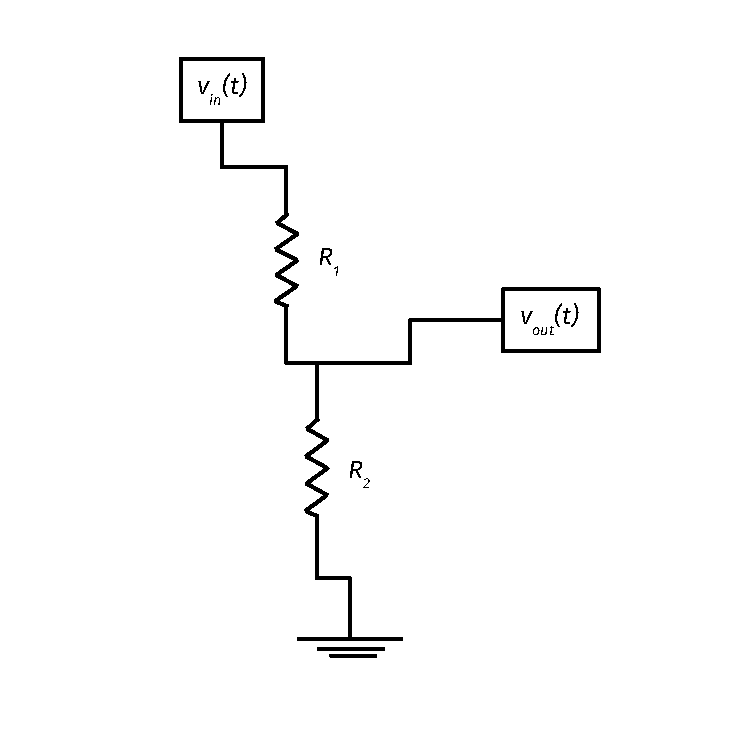
\includegraphics[width=0.5\textwidth,trim=0cm 1cm 0cm 0cm,clip=true]{VoltageDivider.pdf}
\caption{\label{fig:fig1} A two-resistor voltage divider.}
\end{figure}

The input and output voltages with respect to ground must both follow Ohm's law, where $i(t)$ is the current:

\begin{equation}
v_{in} (t) = (R_1 + R_2)i(t)
\label{eq:eq3}
\end{equation}

\begin{equation}
v_{out} (t) = (R_2)i(t)
\label{eq:eq4}
\end{equation}

The resistances $R_1$ and $R_2$ do not depend on frequency.  Taking the Fourier transform of both sides of Eqs. \ref{eq:eq3} and \ref{eq:eq4}, and dividing Eq. \ref{eq:eq4} by Eq. \ref{eq:eq3}, we have

\begin{equation}
\boxed{
\frac{\tilde{v}_{out}(\omega)}{\tilde{v}_{in}(\omega)} = \frac{R_2}{R_1+R_2} \frac{i(\omega)}{i(\omega)} = \frac{R_2}{R_1+R_2}
}
\label{eq:trans1}
\end{equation}

The ratio of output voltage to input voltage is sometimes named the \textit{transfer function.}  In this case, the transfer function only affects the overall amplitude of the output signal, while not affecting any particular frequency, nor shifting any phases.  A circuit in which the resistor labelled $R_2$ has been replaced with a capacitor labelled $C$ is shown in Fig. \ref{fig:fig2}.

\begin{figure}
\centering
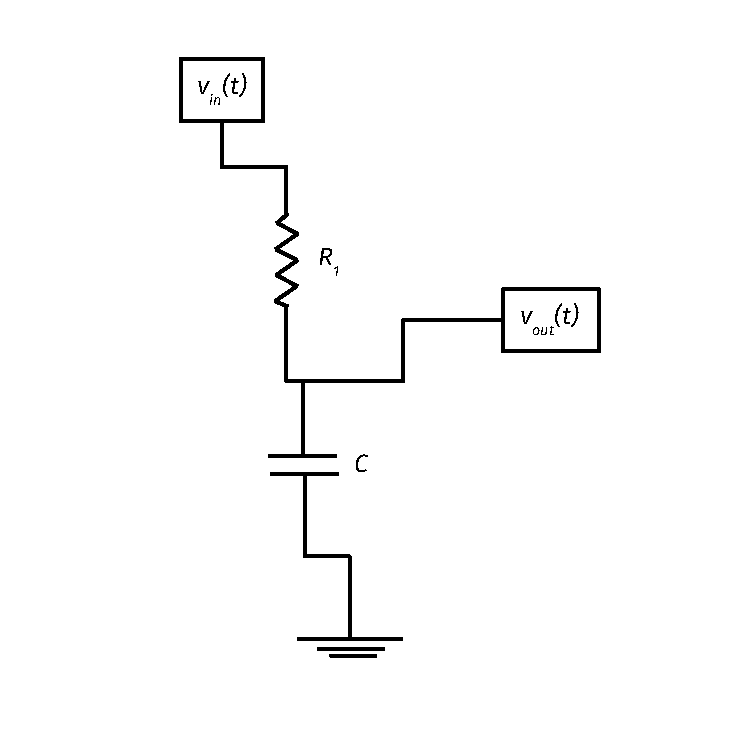
\includegraphics[width=0.5\textwidth,trim=0cm 1cm 0cm 0cm,clip=true]{LowPass.pdf}
\caption{\label{fig:fig2} A frequency-dependent voltage divider, also known as a single-pole RC low-pass filter.}
\end{figure}

The capacitance $C$ is a constant, defined as the ratio of the charge stored on the capacitor, $q$, to the voltage required to place that charge on the capacitor, $V$:

\begin{align}
C &= \frac{q}{V} \\
VC &= q \\
C \frac{dV}{dt} &= \frac{dq}{dt} = i(t) \\
\tilde{i}(\omega) &= j\omega C \tilde{V}(\omega) \\
\frac{\tilde{V}(\omega)}{\tilde{i}(\omega)} &= \frac{1}{j\omega C}
\end{align}

Thus, Ohm's law says that the frequency-dependent resistance, or \textit{impedance}, of a capacitor is

\begin{equation}
\boxed{
Z_C = \frac{1}{j\omega C}
}
\label{eq:eq5}
\end{equation}

The transfer function of the RC circuit in Fig. \ref{fig:fig2} is the same as Eq. \ref{eq:trans1}, with $R_2$ replaced with $Z_C$ (and $R_1 = R$):

\begin{equation}
\frac{\tilde{v}_{out}(\omega)}{\tilde{v}_{in}(\omega)} = \frac{\frac{1}{j\omega C}}{R+\frac{1}{j\omega C}} = \frac{1}{j\omega R C + 1}
\label{eq:trans2}
\end{equation}

Let the \textit{time-constant} be defined as $\tau = RC$, and $\omega_0 = 1/\tau$.  Equation \ref{eq:trans2} may be written:

\begin{equation}
\frac{\tilde{v}_{out}(\omega)}{\tilde{v}_{in}(\omega)} = -\frac{j\omega_0}{\omega - j\omega_0}
\label{eq:eq6}
\end{equation}

The magnitude and phase of Eq. \ref{eq:eq6} are

\begin{equation}
\boxed{
M_{LP}(\omega) = \sqrt{\frac{\omega_0^2}{\omega^2+\omega_0^2}}
}
\label{eq:eq7}
\end{equation}

\begin{equation}
\boxed{
\phi_{LP}(\omega) = -\tan^{-1}\left(\frac{\omega}{\omega_0}\right)
}
\label{eq:eq8}
\end{equation}

From Eq. \ref{eq:eq7}, we can see that the low-pass transfer function $M_{LP}(\omega)$ attenuates frequencies much larger than $\omega_0$.  From Eq. \ref{eq:eq8}, the circuit introduces a phase-shift that is approximately linear ($-\omega/\omega_0$) for frequencies that are not attenuated.  A final interesting quantity to consider is the \textit{group delay}, defined as the negative derivative of the phase:

\begin{equation}
\boxed{
-\frac{d\phi}{d\omega} = \tau_{LP}(\omega) = \frac{\omega_0}{\omega^2+\omega_0^2}
}
\label{eq:eq9}
\end{equation}

Equation \ref{eq:eq9} shows that frequency modes below $\omega_0$ are delayed in time by a factor of $\approx \omega_0^{-1}$.  A final simple circuit to consider is the same as Fig. \ref{fig:fig2}, with the capacitor and resistor exchanged (Fig. \ref{fig:fig3}).  Following the same arguments as the low-pass case, the complex transfer function is

\begin{equation}
\frac{\tilde{v}_{out}(\omega)}{\tilde{v}_{in}(\omega)} = \frac{\omega}{\omega - j\omega_0}
\label{eq:trans3}
\end{equation}

\begin{figure}
\centering
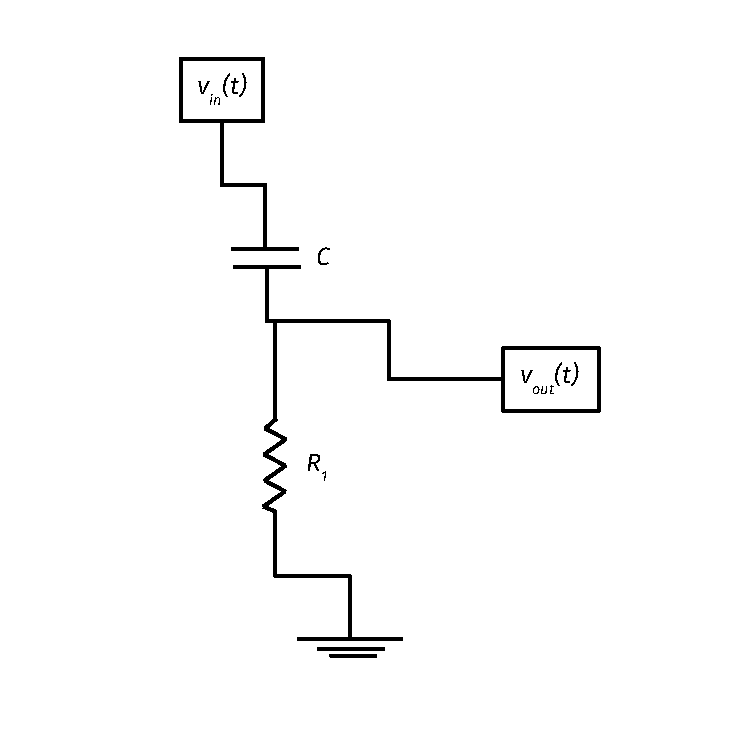
\includegraphics[width=0.5\textwidth,trim=0cm 1cm 0cm 0cm,clip=true]{HighPass.pdf}
\caption{\label{fig:fig3} A frequency-dependent voltage divider, also known as a single-pole RC high-pass filter.}
\end{figure}

The magnitude and phase of Eq. \ref{eq:trans3} are

\begin{equation}
\boxed{
M_{HP}(\omega) = \sqrt{\frac{\omega^2}{\omega^2+\omega_0^2}}
}
\label{eq:eq11}
\end{equation}

\begin{equation}
\boxed{
\phi_{HP}(\omega) = \tan^{-1}\left(\frac{\omega_0}{\omega}\right)
}
\label{eq:eq12}
\end{equation}

The group-delay turns out to be the same as Eq. \ref{eq:eq9}

\begin{equation}
\boxed{
-\frac{d\phi}{d\omega} = \tau_{HP}(\omega) = \frac{\omega_0}{\omega^2+\omega_0^2}
}
\label{eq:eq13}
\end{equation}

Unlike the voltage divider in Fig. \ref{fig:fig1}, which has zero group delay, the circuits in Figs. \ref{fig:fig2} and \ref{fig:fig3} have capacitors.  The group delay in these cases is driven by how quickly these capacitors can be charged and discharged, regardless of where they are in the circuit.

\subsection{Poles and Zeros}

Notice that Eqs. \ref{eq:trans2} and \ref{eq:trans3} become infinite if the frequency is treated as a complex number, with the value $\omega = j\omega_0$.  Treating the frequency as a complex number is useful for further analysis using \textit{contour integration}, allowing us to perform integrals with singularities.  A complex frequency that makes the transfer functions infinite is called a \textit{pole}, and a frequency that makes the transfer functions zero is called a \textit{zero}.  Both the low-pass and high-pass filter examples above have just one pole each.  The low-pass filter has a zero whenever $|\omega| \rightarrow \infty$, and the high-pass filter has a zero for $\omega = 0$.  This is why these circuits are named \textit{single-pole} low and high-pass filters.

\section{Summary of Simple Circuits}

The key results so far may be summarized:

\begin{itemize}
\item The \textit{transfer function} of a circuit may be defined as the ratio of the output voltage to the input voltage in the Fourier domain.
\item The transfer function of a \textit{voltage divider} is given by Eq. \ref{eq:trans1}, a frequency-independent ratio with no phase shift.
\item The transfer function of a \textit{single-pole low-pass filter} is given by Eq. \ref{eq:trans2}.  Magnitude: Eq. \ref{eq:eq7} Phase: Eq. \ref{eq:eq8}
\item The transfer function of a \textit{single-pole high-pass filter} is given by Eq. \ref{eq:trans3}.  Magnitude: Eq. \ref{eq:eq11} Phase: Eq. \ref{eq:eq12}
\end{itemize}

\section{Building a Passive Differentiator}

Consider a single-pole high pass filter, with transfer function given by Eq. \ref{eq:trans3}.  Choose a value for $\omega_0$ much larger than any frequency in the expected input signal: $\omega_0 \gg \omega$.  The transfer function is approximately:

\begin{equation}
\frac{\tilde{v}_{out}(\omega)}{\tilde{v}_{in}(\omega)} \approx \frac{\omega}{-j\omega_0} = j\omega \tau = j\omega RC
\label{eq:eq19}
\end{equation}

Rearranging Eq. \ref{eq:eq19}, and switching back to the time-domain:

\begin{align}
\tilde{v}_{out}(\omega) &\approx j\omega \tau \tilde{v}_{in}(\omega) \\
v_{out}(t) &\approx \tau \frac{dv_{in}}{dt}
\label{eq:eq20}
\end{align}

Equation \ref{eq:eq20} shows that with the correct choice of resistance and capacitance, the circuit output is the derivative of the input, with a \textit{gain} equal to $\tau = RC$.  This circuit is known as a \textit{passive differentiator}.

\section{Building a Passive Integrator}

Consider a single-pole low-pass filter, with transfer function given by Eq. \ref{eq:trans2}.  Choose a value for $\omega_0$ much smaller than any frequency in the expected input signal: $\omega_0 \ll \omega$.  The transfer function is approximately:

\begin{equation}
\frac{\tilde{v}_{out}(\omega)}{\tilde{v}_{in}(\omega)} \approx \frac{-j\omega_0}{\omega}
\label{eq:eq21}
\end{equation}

Rearranging Eq. \ref{eq:eq21}, switching back to the time-domain, and integrating both sides:

\begin{align}
j\omega \tilde{v}_{out}(\omega) &\approx \omega_0 \tilde{v}_{in}(\omega) \\
\frac{dv_{out}}{dt} &= \omega_0 v_{in}(t) \\
v_{out}(t) &= \frac{1}{RC} \int_{t_1}^{t_2} v_{in}(t) dt
\label{eq:eq22}
\end{align}

Equation \ref{eq:eq22} shows that with the correct choice of resistance and capacitance, the circuit output is the integral of the input between two set times, with a \textit{gain} equal to $1/RC$.  This circuit is known as a \textit{passive integrator}.

\section{Summary of Passive Differentiator and Integrator}

\begin{itemize}
\item By choosing a large value of $RC$, relative to input frequencies, the output of a single-pole high-pass filter is proportional to the derivative of the input, with gain $RC$.
\item By choosing a small value of $RC$, relative to input frequencies, the output of a single-pole low-pass filter is proportional to the integral of the input, with gain $1/RC$.
\end{itemize}

\section{Bonus: Circuits with Inductors}

An \textit{inductor} is a circuit-component that stores energy in an internal magnetic field.  The definition of \textit{inductance} is the amount of internal magnetic flux, $\phi$, generated due to a change in the current, $i(t)$:

\begin{equation}
L = \frac{d\phi}{di}
\label{eq:eq14}
\end{equation}

Applying the chain rule to the right-hand side, and applying Faraday's Law of Induction ($d\phi/dt = v$):

\begin{equation}
L = \frac{d\phi}{dt}\frac{dt}{di} = v\frac{dt}{di} = v/i(t)
\label{eq:eq15}
\end{equation}

Faraday's Law of Induction, in this case, states that a voltage $v$ appears in circuits that causes the ensuing current to preserve the internal magnetic field.  Solving for the voltage, and taking the Fourier transform of both sides:

\begin{equation}
\tilde{v}(\omega) = j\omega L \tilde{i}(\omega)
\label{eq:eq16}
\end{equation}

Thus, the impedance of an inductor is 

\begin{equation}
\boxed{
Z_L = j\omega L
}
\label{eq:eq17}
\end{equation}

An example of a circuit comprised of an inductor and a capacitor is shown in Fig. \ref{fig:fig4}.  Following the voltage-divider example, but with $Z_L = j\omega L$ and $Z_C = 1/j\omega C$, we find the transfer function is real:

\begin{equation}
\frac{\tilde{v}_{out}(\omega)}{\tilde{v}_{in}(\omega)} = \frac{1}{1-\omega^2 LC}
\label{eq:eq18}
\end{equation}

\begin{figure}
\centering
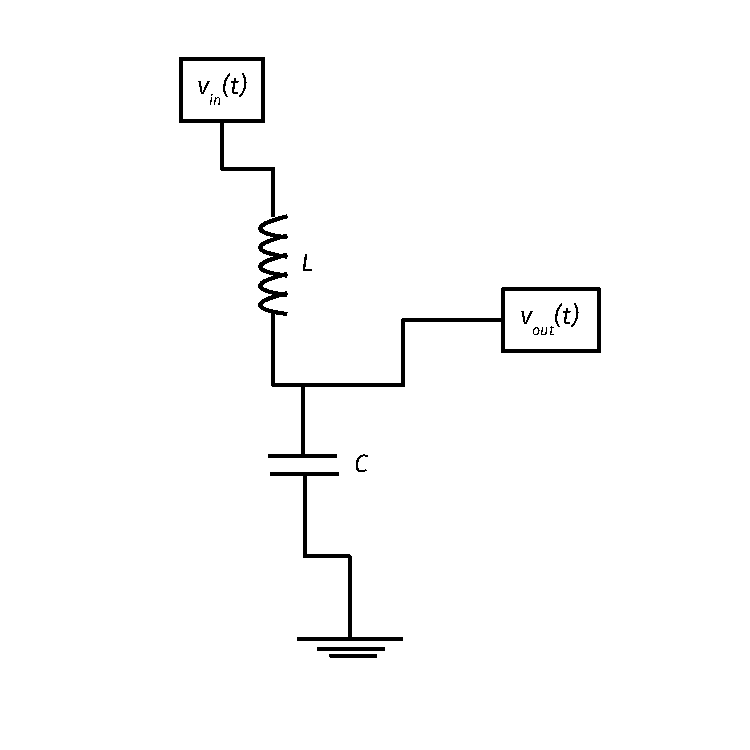
\includegraphics[width=0.5\textwidth,trim=0cm 1cm 0cm 0cm,clip=true]{LowPassLC.pdf}
\caption{\label{fig:fig4} A simple LC-resonator (two-pole).}
\end{figure}

Define a \textit{resonance frequency} $\omega_R^{-2} = LC$, so that 

\begin{equation}
\boxed{
\frac{\tilde{v}_{out}(\omega)}{\tilde{v}_{in}(\omega)} = \frac{\omega_R^2}{\omega_R^2-\omega^2} = \frac{\omega_R^2}{(\omega_R-\omega)(\omega_R + \omega)}
}
\label{eq:trans4}
\end{equation}

The DC value at $\omega = 0$ of the transfer function is 1, and the transfer function approaches zero in the limit of $\omega \gg \omega_R$.  Thus, it is tempting to think of this circuit as a two-pole low-pass filter.  However, for $\omega \approx \omega_R$, the magnitude (absolute value) of the transfer function also approaches infinity.  Thus, we can think of this circuit as more of a \textit{resonator}, rather than a pure filter.  Finally, there is a 180-degree phase-shift if the frequency is greater than the resonance frequency.

\section{Bonus: Summary of RL Circuit}

The key results of the prior section are as follows:

\begin{itemize}
\item The transfer function of a \textit{two-pole RL resonator} is given by Eq. \ref{eq:trans4}.
\item The magnitude of Eq. \ref{eq:trans4} approaches infinity for $\omega \approx \omega_R$
\item The output phase flips by $\pi$ relative to the input phase, depending on whether $\omega > \omega_R$ or $\omega < \omega_R$.
\end{itemize}

\end{document}